% !TeX spellcheck = en_GB
% !TeX TXS-program:compile = txs:///xelatex/[--shell-escape]
% !TeX root = ../build/l2-state-storage.tex




\section{Keys and Values}

In the context of managing key-value data within a Merkle tree structure, it is important to correctly specify the process by which keys and values are employed to create and position data within the tree. The leaf nodes serve as the endpoints of the tree and essentially hold data.

\subsection{Obtaining the Keys}

The current methodology employed for hashing the leaf data to derive the node's key unfolds as follows:

$$ \texttt{leafKey} = \texttt{Poseidon}(\texttt{capacityHash}; \texttt{addr}, 0, \texttt{SMT\_KEY}, 0) $$

The array

$$ \texttt{addr} = (\texttt{addr[0]}, \texttt{addr[1]}, \texttt{addr[2]}, \texttt{addr[3]}, \texttt{addr[4]}) $$

comprises a 32-bit segmented representation of the Ethereum address associated with the leaf, having $160$ bits in the EVM. $\texttt{SMT\_KEY}$ is a single field element that takes the following values for the different L2
state information being stored:

\begin{itemize}
\item \texttt{SMT\_KEY = 0}: for the account balances.
\item \texttt{SMT\_KEY = 1}: for the account nonces.
\item \texttt{SMT\_KEY = 2}: for the smart contracts' code.
\item \texttt{SMT\_KEY = 3}: for the smart contracts' storage.
\item \texttt{SMT\_KEY = 4}: for the smart contracts' length.
\end{itemize}

The computation of the capacity hash differs depending on whether we are storing a storage slot or some other type of data.

\begin{enumerate}[(a)]

\item When storing data that is not a storage slot, the capacity hash is computed as follows:
\[
\texttt{capacityHash}  = \texttt{Poseidon}(\texttt{0}; 0, 0, 0, 0, 0, 0, 0, 0),
\]
where the capacity shown as \texttt{0} is an array of $4$ field elements all of them set to $0$.

\item Since a single smart contract's address can have multiple storage slots, we create different keys for each slot as follows:
\[
\texttt{capacityHash} = \texttt{Poseidon}(\texttt{0}; \texttt{storageKey}),
\]
where \texttt{storageKey} is an array of $8$ field elements where each of these elements is constrained to values of $32$ bits for the representation of the storage slot identifiers, which in the EVM have a size of $256$-bits.

\end{enumerate}


\subsection{Obtaining the Values}

Having specified the procedure for deriving the keys associated with the leaves, it is equally important to outline the process by which the values stored within these leaves are obtained. The current methodology employed for hashing the leaf data to derive the node's value unfolds as follows:
\[
\texttt{leafValue} = \texttt{Poseidon}(\texttt{1}; \texttt{remLeafKey}, \texttt{valueHash}).
\]

In this case, the capacity $\texttt{1}$ is an array of 4 field elements with $\texttt{c}[0] = 1$ and $\texttt{c}[1] = \texttt{c}[2] = \texttt{c}[3] = 0$. The \texttt{remLeafKey} argument of the hash consists as an array of $4$ field elements, which collectively represent the remaining key associated with the leaf node. The second argument \texttt{valueHash} is is an array of 4 field elements that is calculated as follows:
\[
\texttt{valueHash} = \texttt{Poseidon}(\texttt{0}; \texttt{value}),
\]
where $\texttt{value}$ is an array of 8 field elements, with each element constrained to values of 32 bits. The $32$-bits values in the array are computed differently depending on the type of the data intended for storage within the tree.:

\begin{itemize}

\item \textbf{\texttt{balances}, \texttt{nonces} and \texttt{storageSlotValues}.}

In the EVM, \texttt{balances}, \texttt{nonces} and \texttt{storageSlotValues} are of $256$ bits. So, their \texttt{valueHashes} are computed as expected:
\begin{align*}
\texttt{valueHash} &= \texttt{Poseidon(0; balance)}, \\
\texttt{valueHash} &= \texttt{Poseidon(0; nonce)}, \\
\texttt{valueHash} &= \texttt{Poseidon(0; storageSlotValue)}.
\end{align*}

All the previous arrays are of 8 field elements constrained to values of 32 bits.

\item \textbf{Smart Contracts Code.}

In the L2 state tree we also need to store the hash of the smart contracts’ bytecode. The issue is that the bytecode of smart contract can be larger than $256$-bits ($32$ bytes). Actually, it can have an arbitrary size. To manage these issues:

\begin{itemize}

\item We use a \textbf{padding} to complete the size of data being hashed to a multiple of a suitable size that is $56$ bytes (we see why next).

\item Then, we linearly hash the resulting padded byte string.

\end{itemize}

\begin{figure}[H]
\centering
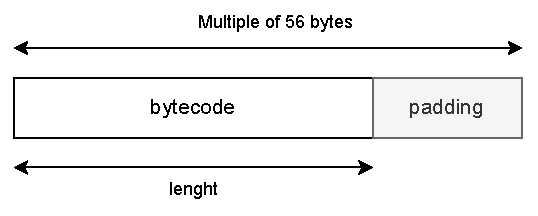
\includegraphics[width=0.5\columnwidth]{\zkevmdir/figures/architecture/L2StateTree/bytecode-padding.drawio}
\caption{The padding is introduced in order to enable the bytecode to be hashed using \texttt{Poseidon}. }
\label{fig:padding}
\end{figure}
In the L2 state tree, we also need to store the bytecode length to distinguish what is payload from what is padding:

\begin{itemize}

\item The bytecode length represents the number of bytes of the bytecode.

\item This is a 256-bit value.

\item The \texttt{valueHash} is computed as follows:
\[
\texttt{valueHash} = \texttt{Poseidon(0;} \texttt{bytecodeLength}).
\]

\end{itemize}

We encode the bytecode (which is multiple of a byte) in segments of 7 bytes (56 bits), which is the biggest amount of bytes that can be represented with an element of our field:
\[
2^{56} < 2^{64} - 2^{32} + 1 < 2^{64}.
\]

The \texttt{Poseidon} hash function signature that use has 8 inputs, so we hash in blocks of 8 field elements which encode $7\,$ bytes $\times\, 8\,$ elements $= 56$ bytes of bytecode. So, we use a padding procedure that completes the original bytecode string to a padded string that is multiple of 56 bytes as follows:

\begin{enumerate}
\item Add the byte \texttt{0x01} at the end of the original bytecode.
\item Fill with zeros until the padded bytecode length + 1 is multiple of 56 bytes.
\item Add \texttt{0x80} as the last byte.
\end{enumerate}

For example, if the original bytecode is \texttt{0xdead}, having size of $2$ bytes, the padded bytecode becomes \texttt{0xdead01000000000000000000...000000000000080}, having size of $56$ bytes.

Since smart contract's bytecode can be larger than $256$ bits, we will need a chained hash process in order to obtain a valid representative value (that we will call \texttt{bytecodeHash}). More specifically, we recursively hash $8$ of the $7$ bytes segments along with the hash of the preceding chunk, input as the capacity element.

\begin{figure}[H]
\centering
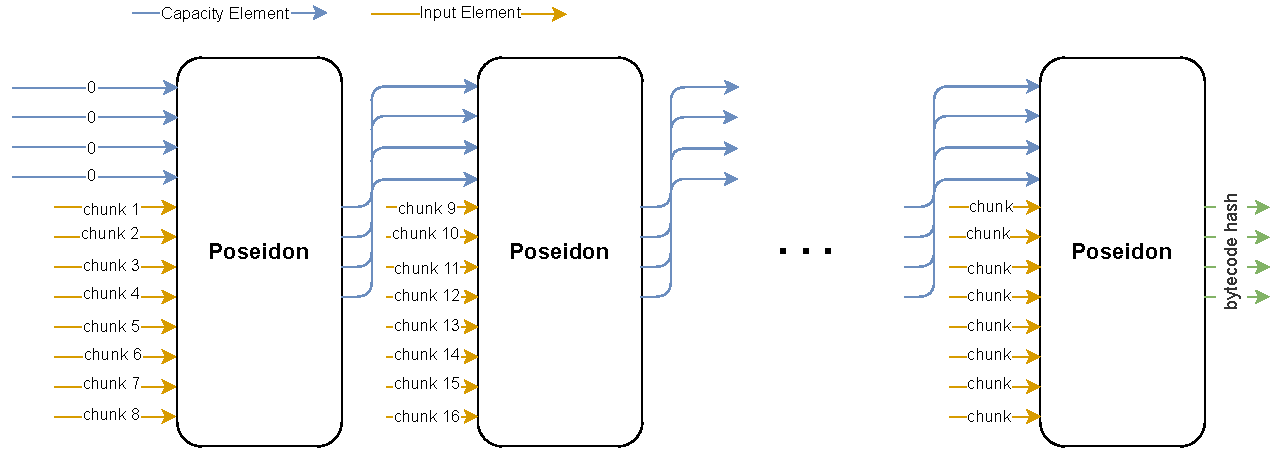
\includegraphics[width=.9\columnwidth]{\zkevmdir/figures/architecture/L2StateTree/bytecode-linear-hash.drawio}
\caption{Notice that we use the output of the previous \texttt{Poseidon} function as the capacity in the new computation of the next \texttt{Poseidon} hash.}
\label{fig:linear-hash}
\end{figure}

Following the previous example having \texttt{0xdead} as the bytecode. Recall that the padded bytecode became
\[
\texttt{0xdead010000000000000000000000000...000000000000000000000080}.
\]
We perform one \texttt{Poseidon} (since the padded bytecode has length $56$ bytes) with the following $12$ elements:

\begin{figure}[H]
\centering
\begin{lstlisting}[style=verbtt]
[ "00000000000000", (7 bytes) (element 0)
  "00000000000000", (7 bytes) (element 1)
  "00000000000000", (7 bytes) (element 2)
  "00000000000000", (7 bytes) (element 3)
  "0000000001adde"  (7 bytes) (element 4)
  "00000000000000"  (7 bytes) (element 5)
  "00000000000000"  (7 bytes) (element 6)
  "00000000000000"  (7 bytes) (element 7)
  "00000000000000"  (7 bytes) (element 8)
  "00000000000000"  (7 bytes) (element 9)
  "00000000000000"  (7 bytes) (element 10)
  "80000000000000"  (7 bytes) (element 11) ]
\end{lstlisting}
\caption{The \texttt{Poseidon} hash is performed with 12 elements, each representing a 7-byte value. Since we are performing the first $7$ bytes, we leave the capacity to $\texttt{0}$. }
\label{fig:example}
\end{figure}

Finally, the \texttt{valueHash} of the bytecode is  \texttt{valueHash} = \texttt{Poseidon(0;} \texttt{bytecodeHash}).

\end{itemize}